\section*{Chapter 4: Results and Discussion}
\setcounter{section}{4} \setcounter{subsection}{0}
\addcontentsline{toc}{section}{\textit{Chapter 4: Results and Discussion}}
\phantomsection \label{chap:evaluation}

\texttt{linux-mcp} is evaluated along four dimensions: control-plane latency and its breakdown across invocation stages, throughput under concurrent load, resistance to a representative set of control-plane attacks, and system behaviour under daemon failure and restart.
The central claim under test is that relocating admission-control state into the kernel strengthens enforcement without making the tool invocation path prohibitively expensive.
Two baselines isolate this effect from user-space hardening alone: a conventional user-space mediator (\textbf{userspace}), in which registration, admission, and approval all reside in the daemon, and a hardened variant (\textbf{seccomp}) that augments the same control path with stricter syscall filtering, additional validation, and audit logging.

The prototype under test comprises 43 tools across 14 applications; all three systems operate over this same tool deployment throughout the evaluation.
All experiments were conducted on a VMware guest (Apple aarch64 host, 4 vCPU, 8 GB RAM) in a headless configuration with no concurrent user-space workloads.
Latency results are reported over $n = 30$ independent runs of 2000 requests each, giving a standard error of the mean small enough to support Welch's $t$-test comparisons at $\alpha = 0.05$ while remaining within the hypervisor timing noise of a virtualised guest.
Throughput and the category-level security evaluation are drawn from the same run, using the harness's built-in concurrency sweep and ten repeats of each attack case.
All reported $p$-values are two-sided Welch's $t$-tests \cite{west2021welch} comparing per-repetition mean latency against the \texttt{userspace} baseline.


\subsection{Latency and Control-Plane Overhead}

Table~\ref{tab:latency} and Figure~\ref{fig:chapter4-latency} report mean end-to-end latency for each system at three payload sizes.
The 100~B and 10~KB points correspond to typical MCP tool invocations (short JSON commands and small structured responses), while the 1~MB point is a contrived stress case rather than a representative workload: it is used solely to probe how the control plane behaves when the payload dominates the cost of a request, and is not intended to reflect everyday tool traffic.
At 100~B, the kernel path and the user-space baseline are within measurement noise: both at \num{0.854}~ms ($p = 0.984$).
At 10~KB the kernel path is nominally slower (\num{0.899}~ms versus \num{0.863}~ms, +4.2\%), but the difference does not reach significance ($p = 0.097$), a sub-millisecond effect lost in the timing noise of a VMware guest at $n = 30$.

\begin{table}[!htbp]
\centering
\caption{Mean end-to-end latency (ms) by payload size ($n = 30$ runs $\times$ 2000 requests). Bold values indicate the lowest latency per row. $p$-values are two-sided Welch's $t$-tests against the \texttt{userspace} baseline; \textsuperscript{ns} = not significant ($p > 0.05$).}
\label{tab:latency}
\setlength{\tabcolsep}{8pt}
\renewcommand{\arraystretch}{1.25}
\begin{tabular}{lrrr@{\hspace{14pt}}rr}
\toprule
& \multicolumn{3}{c}{\textbf{Mean latency (ms)}}
& \multicolumn{2}{c}{\textbf{Welch's $p$-value}} \\
\cmidrule(lr){2-4}\cmidrule(lr){5-6}
\textbf{Payload}
  & \texttt{userspace}
  & \texttt{seccomp}
  & \texttt{kernel}
  & vs.\ \texttt{seccomp}
  & vs.\ \texttt{kernel} \\
\midrule
\rowcolor{gray!8}
100\,B  & \textbf{0.854} & 0.867 & \textbf{0.854} & 0.475\textsuperscript{ns}  & 0.984\textsuperscript{ns} \\
10\,KB  & 0.863          & 0.922 & 0.899          & 0.000206                  & 0.097\textsuperscript{ns} \\
\rowcolor{gray!8}
1\,MB   & 7.748          & 9.843 & \textbf{7.487} & ${<}10^{-4}$              & 0.00027 \\
\bottomrule
\end{tabular}
\end{table}

\begin{figure}[!htbp]
\centering
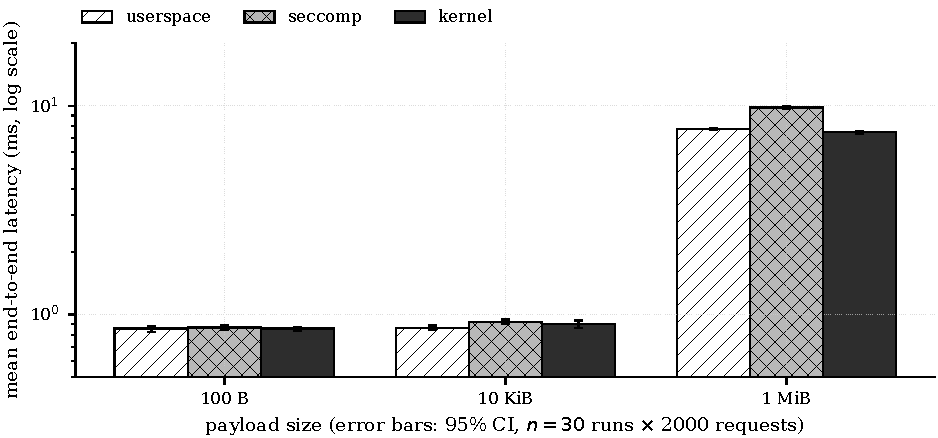
\includegraphics[width=0.98\linewidth]{figures/figure_latency_mean_by_payload.pdf}
\caption{Mean end-to-end latency by payload size for the three systems. Each subplot auto-scales its own y-axis so that the sub-millisecond differences at 100~B and 10~KB are not flattened by the much larger absolute values at 1~MB.
Error bars show 95\% confidence intervals across $n = 30$ independent runs; significance markers are Welch's $t$-test against the \texttt{userspace} baseline.}
\label{fig:chapter4-latency}
\end{figure}

The 1~MB result is the one definitive number in the table.
The kernel path runs at \num{7.487}~ms, compared to \num{7.748}~ms for plain user-space (a 3.4\% reduction, $p = 0.00027$) and \num{9.843}~ms for the hardened variant.
This is counter-intuitive: adding a privilege boundary is usually expected to cost latency, not return it.
Figure~\ref{fig:chapter4-overhead} shows the same data as a ratio against the plain \texttt{userspace} baseline, with the y-axis zoomed around the parity line so that the sub-4\% effects at 100~B and 10~KB are visible in the same frame as the larger effect at 1~MB; read that way, \texttt{seccomp} sits above parity at every payload size while the kernel path crosses below parity only at 1~MB.
The explanation has two parts.
The seccomp penalty at large payloads is the accumulating cost of BPF per-syscall filtering across the heavier socket traffic that a megabyte payload forces through, and the kernel path does not pay that cost at all.
The modest speedup against plain user-space, we believe, reflects early-reject behaviour: arbitration happens before the payload is copied through the tool-forwarding socket, so a rejected request avoids a copy the user-space baseline would still have to perform between admission and forwarding.

\begin{figure}[!htbp]
\centering
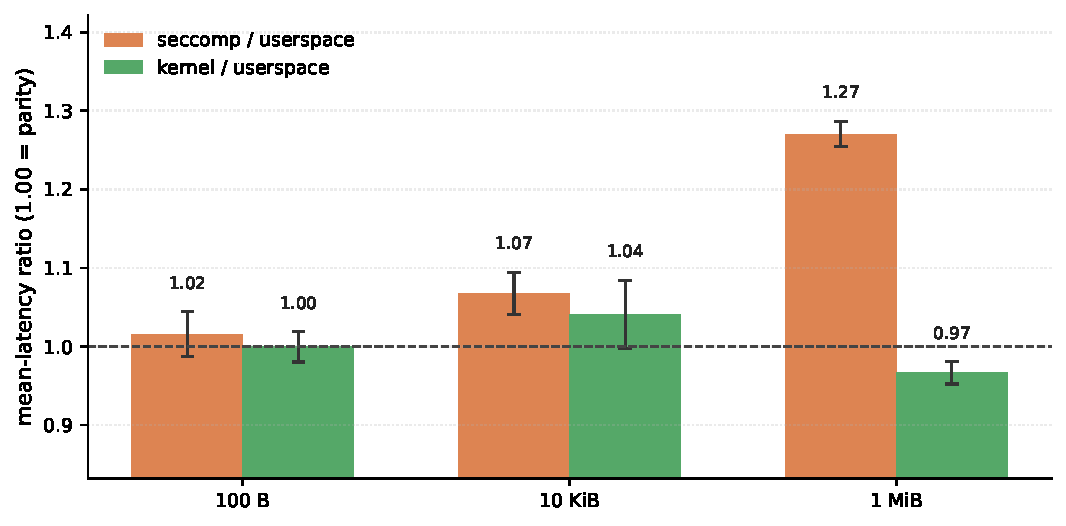
\includegraphics[width=0.95\linewidth]{figures/figure_latency_overhead.pdf}
\caption{Mean-latency ratio of each hardened variant to the plain \texttt{userspace} baseline, with 95\% confidence intervals propagated from the 30-run per-repetition means. The y-axis is zoomed around the parity line (ratio = 1.00) to make the sub-4\% effects at 100~B and 10~KB visible alongside the larger effect at 1~MB. The \texttt{seccomp} path is significantly slower at every payload size; the \texttt{kernel} path is statistically indistinguishable from \texttt{userspace} at small and medium payloads and measurably faster at 1~MB.}
\label{fig:chapter4-overhead}
\end{figure}

The $p_{95}$ picture, shown in Figure~\ref{fig:chapter4-p95}, matches the means.
At 100~B and 10~KB the three systems are statistically indistinguishable ($p = 0.51$ and $p = 0.16$).
At 1~MB the kernel $p_{95}$ is \num{8.422}~ms, against \num{8.716}~ms for user-space ($p = 0.049$) and \num{10.903}~ms for seccomp.
The tail does not widen under the enforcement boundary.

\begin{figure}[!htbp]
\centering
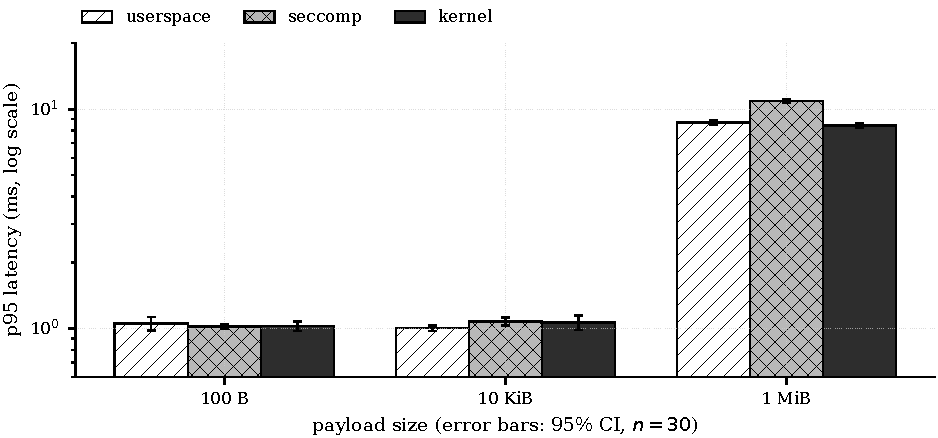
\includegraphics[width=0.98\linewidth]{figures/figure_latency_p95_by_payload.pdf}
\caption{$p_{95}$ latency by payload size for the three systems ($n = 30$ runs of 2000 requests each). Error bars show 95\% confidence intervals. At 100~B and 10~KB the kernel path is statistically indistinguishable from the userspace baseline; at 1~MB the kernel $p_{95}$ (\num{8.422}~ms) is lower than both userspace (\num{8.716}~ms, $p = 0.049$) and seccomp (\num{10.903}~ms), confirming that the enforcement boundary does not widen the tail under the tested workload.}
\label{fig:chapter4-p95}
\end{figure}

Stage-level breakdown in Figure~\ref{fig:chapter4-breakdown} confirms that kernel arbitration is a minor contributor at all payload sizes.
Mean arbitration time is \num{0.028}~ms at 100~B and 10~KB, and \num{0.038}~ms at 1~MB.
At 1~MB, tool execution accounts for \num{89.3}\% of total end-to-end time on the kernel path (\num{89.9}\% on the user-space path); the entire control-plane machinery (Generic Netlink round-trip, session lookup, and arbitration) accounts for the remaining \num{10.7}\%, with the arbitration contribution within that fraction less than four hundredths of a millisecond.

\begin{figure}[!htbp]
\centering
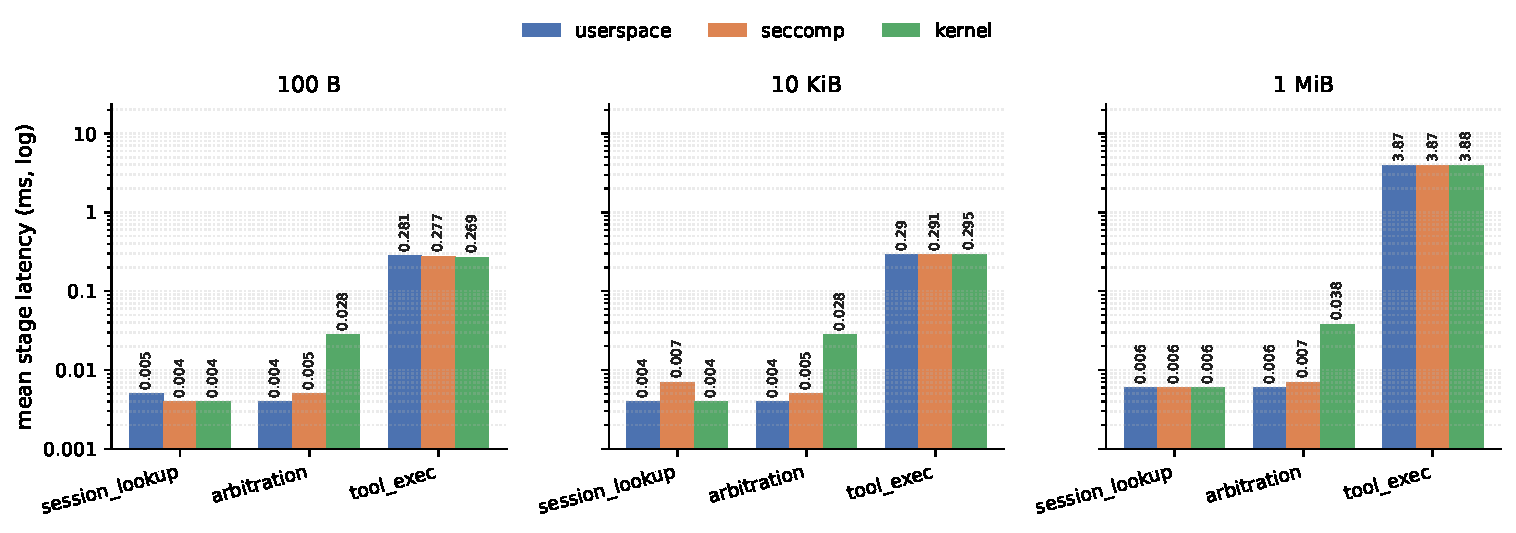
\includegraphics[width=0.98\linewidth]{figures/figure_latency_breakdown.pdf}
\caption{Invocation-stage breakdown (session lookup, arbitration, tool execution) for each system at all three payload sizes, on a log y-axis. The log scale makes session\_lookup (around 4~\textmu s) visible alongside tool\_exec (around 4~ms). The \texttt{kernel} path spends roughly one order of magnitude more time in arbitration than the user-space baselines, but that extra cost is well under \num{0.04}~ms and is invisible relative to the tool-execution component.}
\label{fig:chapter4-breakdown}
\end{figure}

A supplementary microbenchmark isolates the Generic Netlink layer using a minimum-cost \texttt{KMCP\_\allowbreak CMD\_\allowbreak NOOP} handler added to the kernel module.
The NOOP path returns immediately after Generic Netlink demultiplexing, without touching any tool or agent registry, and therefore measures the irreducible floor of a round-trip against which all per-stage arbitration costs can be anchored.
Figure~\ref{fig:chapter4-ablation} reports the medians on a single axis: the NOOP floor sits at \num{3.125}~$\mu$s, the full \texttt{TOOL\_\allowbreak REQUEST} path measured at a realistic registry scale of 1024 tools and 64 agents sits at \num{7.459}~$\mu$s, and the \texttt{skip\_\allowbreak lookups} and \texttt{ticket\_\allowbreak trigger} bars bracket the per-stage contributions that the next paragraph decomposes.
The total kernel arbitration cost is therefore \num{4.334}~$\mu$s above the noise floor, which is roughly one order of magnitude smaller than the sub-millisecond effects visible in the end-to-end measurements; the dominant cost on the kernel path originates in user-space components (session management, payload serialisation, and socket I/O) rather than in the kernel module itself.

\begin{figure}[!htbp]
\centering
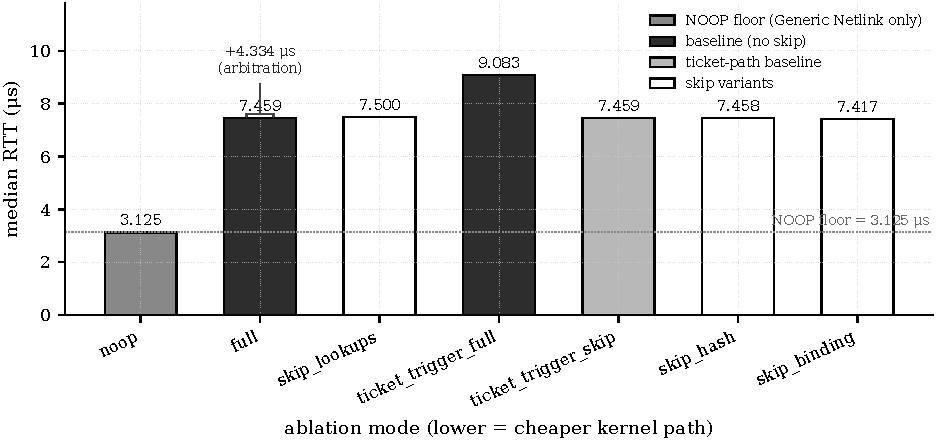
\includegraphics[width=0.95\linewidth]{figures/figure_ablation_mean_rtt.pdf}
\caption{Kernel path ablation at realistic registry scale ($N = 1024$ tools, $M = 64$ agents). The leftmost bar is the measured noise floor from the \texttt{KMCP\_\allowbreak CMD\_\allowbreak NOOP} handler, which establishes the irreducible Generic Netlink round-trip cost. The \texttt{full} bar is the complete \texttt{TOOL\_\allowbreak REQUEST} arbitration path; \texttt{skip\_\allowbreak lookups} disables the tool and agent registry walks. The two \texttt{ticket\_\allowbreak trigger} bars exercise a high-risk tool whose execution is gated by the approval-ticket machinery, with and without the approval branch bypassed. All error bars are 95\% bootstrap CIs across $n = 10$ repetitions.}
\label{fig:chapter4-ablation}
\end{figure}

To decompose the \num{4.334}~$\mu$s arbitration cost into its constituent stages, a paired ablation was performed against compile-time experiment flags that selectively bypass individual kernel code paths (\texttt{SKIP\_\allowbreak LOOKUPS}, \texttt{SKIP\_HASH}, \texttt{SKIP\_\allowbreak BINDING}, \texttt{SKIP\_\allowbreak TICKET}).
Each stage delta is measured by alternating the baseline and bypass modes request-by-request within a single benchmark phase, so the two samples in every pair are collected microseconds apart and share the same scheduler state and cache residency.
Hypervisor-level drift that contaminates naive sequential-mean comparisons cancels out inside the paired difference, and bootstrap CIs on the delta vector are correspondingly tighter.

Table~\ref{tab:ablation-stages} and Figure~\ref{fig:chapter4-ablation-stages} together report the two stages whose guard bodies are actually executed by the benchmark workload, plus two methodology-check rows that document the path-identity caveat.
The \texttt{registry+agent\_\allowbreak lookup} stage (two mutex pairs, an \texttt{xa\_load} against a 1024-entry xarray, and a 64-entry hashtable walk) contributes \num{0.109}~$\mu$s per request.
The \texttt{approval\_\allowbreak ticket\_\allowbreak body} stage (consume plus issue, including an \texttt{approval\_\allowbreak lock} acquisition and hashtable insert) contributes \num{2.012}~$\mu$s per request and is only exercised when the tool is high-risk and the request arrives without a pre-authorised ticket.
Under benign credentials the \texttt{hash} and \texttt{binding} guard bodies are dead code (short-circuited by the workload state before the experiment flag is consulted), and their paired deltas correctly return $0 \pm$ noise with $p_{\text{BH}} > 0.5$, confirming that the paired method introduces no systematic bias on identical code paths.

\begin{table}[!htbp]
\centering
\caption{Paired per-stage ablation deltas. Each row alternates a baseline mode and a bypass mode request-by-request inside a single phase; the $\Delta$ column is the mean of $\text{baseline}_i - \text{bypass}_i$ across all pairs. BH-corrected paired $t$-tests are reported across all four comparisons.}
\label{tab:ablation-stages}
\setlength{\tabcolsep}{5pt}
\renewcommand{\arraystretch}{1.2}
\begin{tabular}{lrrlrr}
\toprule
\textbf{Stage} & $n_{\text{pairs}}$ & $\Delta_{\text{avg}}$ ($\mu$s) & \textbf{95\% CI} ($\mu$s) & $t_{\text{paired}}$ & $p_{\text{BH}}$ \\
\midrule
registry+agent\_lookup & 100\,000 & $+0.109$ & $[+0.087, +0.131]$ & $+10.08$ & $<10^{-4}$ \\
approval\_ticket\_body   & 1\,000   & $+2.012$ & $[+1.760, +2.257]$ & $+15.99$ & $<10^{-4}$ \\
\midrule
\multicolumn{6}{l}{\textit{Methodology consistency checks (dead guard bodies under benign workload)}} \\
hash\_guard\_body        & 100\,000 & $+0.163$ & $[-0.153, +0.541]$ & $+0.88$  & $0.507$ \\
binding\_guard\_body     & 100\,000 & $-0.007$ & $[-0.027, +0.013]$ & $-0.65$  & $0.513$ \\
\bottomrule
\end{tabular}
\end{table}

\begin{figure}[!htbp]
\centering
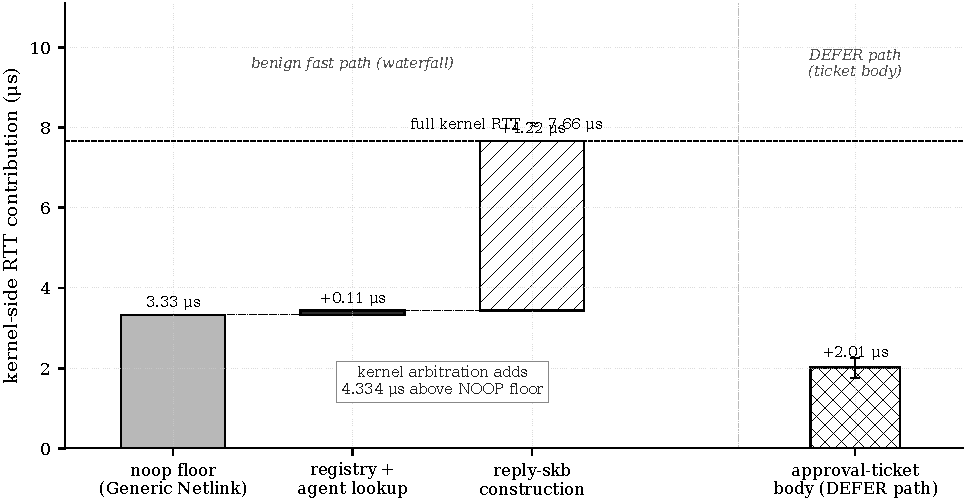
\includegraphics[width=0.95\linewidth]{figures/figure_ablation_stage_delta.pdf}
\caption{Paired per-stage deltas across the four ablation comparisons. The first two bars are the meaningful stage costs (registry+agent lookup and the approval-ticket body); the last two are methodology consistency checks against dead guard bodies and are expected to fall on zero.}
\label{fig:chapter4-ablation-stages}
\end{figure}

Subtracting the \num{0.109}~$\mu$s registry+lookup cost from the \num{4.334}~$\mu$s total leaves roughly \num{4.2}~$\mu$s unattributed in the benign run (the approval-ticket body is not exercised along this path, so its cost does not enter the sum).
The remainder is reply-skb construction: the five \texttt{nla\_put\_*} calls and the \texttt{genlmsg\_\allowbreak reply} in \texttt{kernel\_\allowbreak mcp\_\allowbreak reply\_\allowbreak tool\_\allowbreak decision}, which the experiment flags do not decompose further.

One caveat about the \texttt{approval\_\allowbreak ticket\_\allowbreak body} figure deserves explicit mention.
Every ticket issuance calls \texttt{kernel\_\allowbreak mcp\_\allowbreak purge\_\allowbreak expired\_\allowbreak tickets\_\allowbreak locked()}, which iterates the full 256-bucket approval hashtable.
Under \num{300}~s TTL, no ticket expires during a one-minute microbenchmark, so the purge scan cost grows linearly with the number of tickets the benchmark has already issued.
Moving the expiry scan to the existing periodic \texttt{kernel\_\allowbreak mcp\_\allowbreak ticket\_\allowbreak cleanup\_\allowbreak timer} would eliminate this $O(n)$ component entirely.
This is flagged as a simple future-work optimisation, not a characteristic of the fast path in production use where \texttt{mcpd} consumes tickets promptly and the hashtable stays small.


\subsection{Throughput and Scalability}

Throughput was measured across agent counts $\{1, 5, 10, 20, 50\}$ and concurrency levels $\{1, 10, 50, 100\}$ to check whether the kernel-assisted control plane becomes a bottleneck once multiple requests are in flight simultaneously.
Table~\ref{tab:throughput} gives the per-cell peak throughput at one agent; the complete sweep across agent counts produces the same shape and is summarised in prose below.

\begin{table}[!htbp]
\centering
\caption{Peak throughput (RPS) at one agent, across concurrency levels ($n = 5$ repetitions per cell). The \texttt{userspace} column is the highest in every row; the \texttt{kernel} path sits roughly 10\% below it at every concurrency level, without collapsing.}
\label{tab:throughput}
\setlength{\tabcolsep}{10pt}
\renewcommand{\arraystretch}{1.2}
\begin{tabular}{rrrr}
\toprule
\textbf{Concurrency} & \texttt{userspace} & \texttt{seccomp} & \texttt{kernel} \\
\midrule
\rowcolor{gray!8}
1   & 1117.5 & 1088.5 & 1071.1 \\
10  & 1146.0 & 1036.9 & 1009.4 \\
\rowcolor{gray!8}
50  & 1215.6 & 1123.5 & 1096.2 \\
100 & 1213.4 & 1072.5 & 1103.7 \\
\bottomrule
\end{tabular}
\end{table}

Plain user-space achieves the highest peak throughput in every row, ranging from \num{1090} to \num{1219}~RPS across the full grid.
The kernel path ranges from \num{1003} to \num{1137}~RPS, and the seccomp path from \num{1020} to \num{1200}~RPS.
At a representative operating point of one agent and concurrency 50, the three systems sit at \num{1215.6}, \num{1123.5}, and \num{1096.2}~RPS respectively.
The kernel path is roughly 10\% slower than the user-space peak, which is consistent with the additional Generic Netlink round-trip and with the serialisation of admission decisions through a single kernel module.

These numbers come from an earlier $n = 5$ pilot run.
The $n = 30$ study that drives the latency table was deliberately scoped to latency alone and did not repeat the concurrency sweep, so the throughput figures carry wider uncertainty than the latency figures and should be read as evidence of practical viability rather than as a precise ceiling.
Within the tested range the kernel path holds a stable $\sim$10\% gap without collapsing, which is enough to support the viability claim.
A follow-up sustained-overload run was attempted at concurrencies of 200, 400, and 800, but the \texttt{SOMAXCONN} accept queue saturated before the control plane itself became the bottleneck, so those cells produced error-dominated latency distributions rather than usable p99 curves and are not reported here.


\subsection{Registry Scaling}
\label{sec:registry-scaling}

A separate experiment characterises how the kernel-side tool registry behaves as the catalogue grows beyond the 43-tool deployment used elsewhere in the evaluation.
$N$ synthetic tools (with $N \in \{8, 16, 32, \ldots, 16\,384\}$) are bulk-registered into the kernel, and both the register path and the steady-state lookup path are measured.
The register path is modelled as a one-time setup cost plus a per-tool steady-state cost:
\[
\text{total\_ms}(N) = a + b \cdot N,
\]
fitted across the 12 values of $N$ by ordinary least squares.

The fit produces $a = -0.123$~ms, $b = 6.011$~$\mu$s per tool, and $R^2 = 0.9996$.
The asymptotic registration throughput is therefore $1/b \approx 166\,000$ tools/s; the 43-tool catalogue used in the main evaluation registers in approximately \num{0.26}~ms of wall-clock time, and even a \num{16384}-tool deployment completes its one-shot registration in under \num{100}~ms.
The per-tool cost curve (Figure~\ref{fig:chapter4-registry-curve}) approaches the asymptote $b$ from above with no inflection point --- there is no scaling degradation at large $N$, and the apparent variation at small $N$ is the intercept $a$ amortising away.

\begin{figure}[!htbp]
\centering
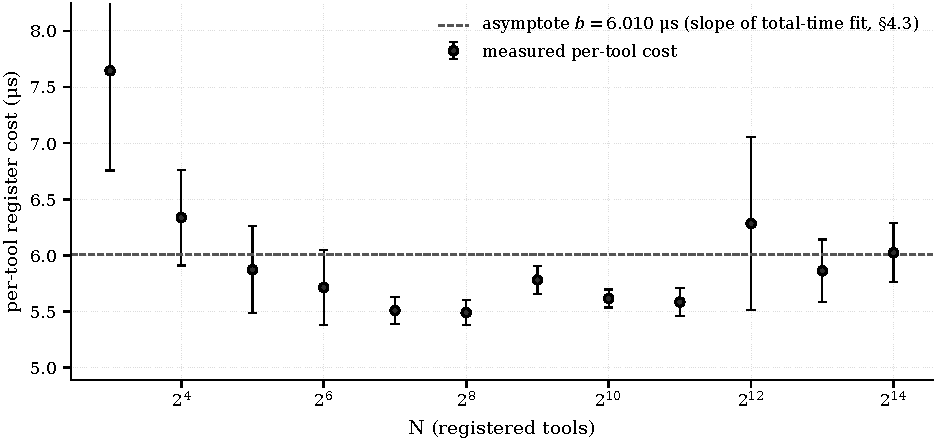
\includegraphics[width=0.95\linewidth]{figures/figure_registry_register_curve.pdf}
\caption{Registry register-path per-tool cost as a function of registry size $N$. The dashed line is the asymptotic per-tool cost $b = 6.011$~$\mu$s from the linear fit $\text{total\_ms}(N) = a + b N$ ($R^2 = 0.9996$); the curve approaches this asymptote monotonically with no degradation at large $N$.}
\label{fig:chapter4-registry-curve}
\end{figure}

The steady-state lookup path is measured separately by drawing a random \texttt{tool\_id} for each request against the pre-populated registry; the log-linear regression $\text{lookup\_ms} \sim a + b \cdot \log_2 N$ produces a slope of \num{2.9e-5}~ms per doubling with a bootstrap 95\% CI of $[-2\times 10^{-6}, +6.1\times 10^{-5}]$ that contains zero ($R^2 = 0.26$).
The near-zero slope and the CI overlapping zero are consistent with the expected $O(1)$ behaviour of the underlying xarray data structure, and inconsistent with any balanced-tree implementation where slope would grow with $\log_2 N$ at high $R^2$.
Figure~\ref{fig:chapter4-registry-lookup} shows the lookup latency distribution across the full range of $N$.
Mean lookup latency stays within the 7.1--7.7~$\mu$s band across three orders of magnitude of registry size.

\begin{figure}[!htbp]
\centering
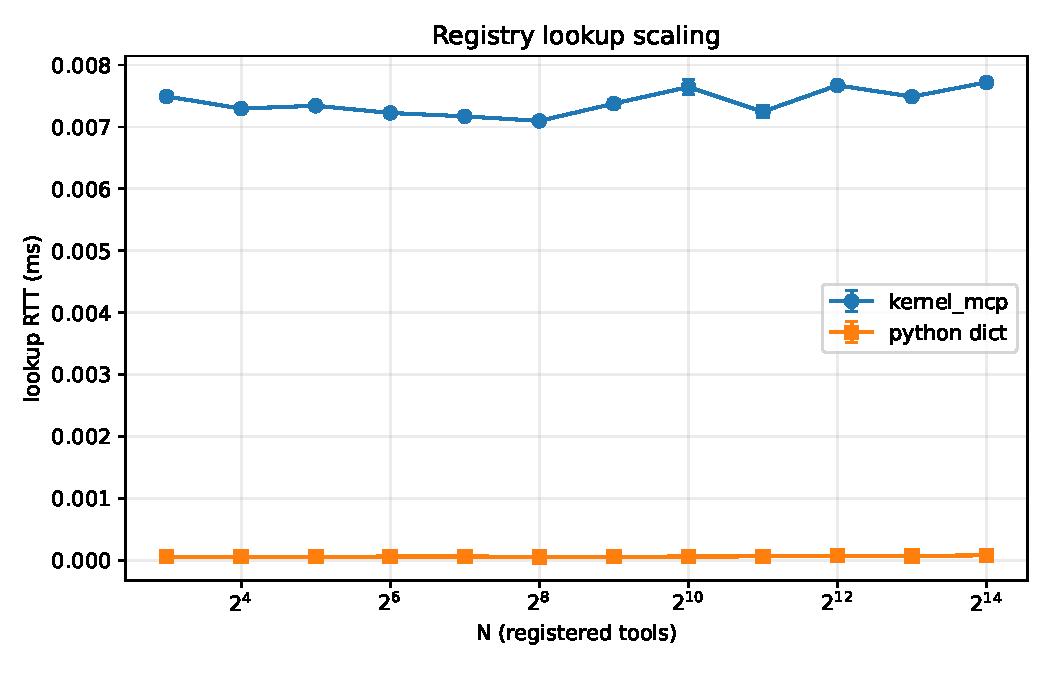
\includegraphics[width=0.95\linewidth]{figures/figure_registry_lookup_scaling.pdf}
\caption{Steady-state \texttt{tool\_id} lookup latency as a function of registry size $N$, on a log-$N$ axis. The fitted log-linear slope is $2.9\times 10^{-5}$~ms per doubling (bootstrap 95\% CI $[-2\times 10^{-6}, +6.1\times 10^{-5}]$, containing zero), consistent with the $O(1)$ xarray lookup invariant.}
\label{fig:chapter4-registry-lookup}
\end{figure}


\subsection{Security Evaluation}

The latency and throughput numbers establish that kernel placement is not prohibitively expensive, but the argument for making the move hinges on whether it actually changes what attackers can do.
The security evaluation targets four categories from the threat model in \hyperref[chap:background]{Chapter~2}: identity spoofing (forging session identity to impersonate a registered agent), replay (reusing a stale approval ticket), substitution (tampering with \texttt{tool\_id} or \texttt{tool\_hash} to redirect execution), and escalation (bypassing the approval gate on a high-risk invocation).

Each system received 110 attack attempts in total (11 distinct cases $\times$ 10 repeats: 3 spoof, 4 replay, 3 substitution, 1 escalation).
Outcomes are summarised in Table~\ref{tab:attacks} and Figure~\ref{fig:chapter4-security}.

\begin{table}[H]
\centering
\caption{Category-level attack outcomes by system (110 attempts each: 3 spoof, 4 replay, 3 substitution, 1 escalation, $\times$ 10 repeats). The bypass rate measures the fraction of attempts that succeeded in circumventing the intended control. The user-space bypass rates reflect deliberate per-category instrumented weakening of the mediator and do not represent the performance of a fully hardened user-space implementation.}
\label{tab:attacks}
\begin{tabular}{lccc}
\toprule
System & Bypasses & Total & Bypass rate \\
\midrule
\texttt{userspace} & 100 & 110 & 90.9\% \\
\texttt{seccomp}   &  40 & 110 & 36.4\% \\
\texttt{kernel}    &   0 & 110 &  0.0\% \\
\bottomrule
\end{tabular}
\end{table}

\begin{figure}[!htbp]
\centering
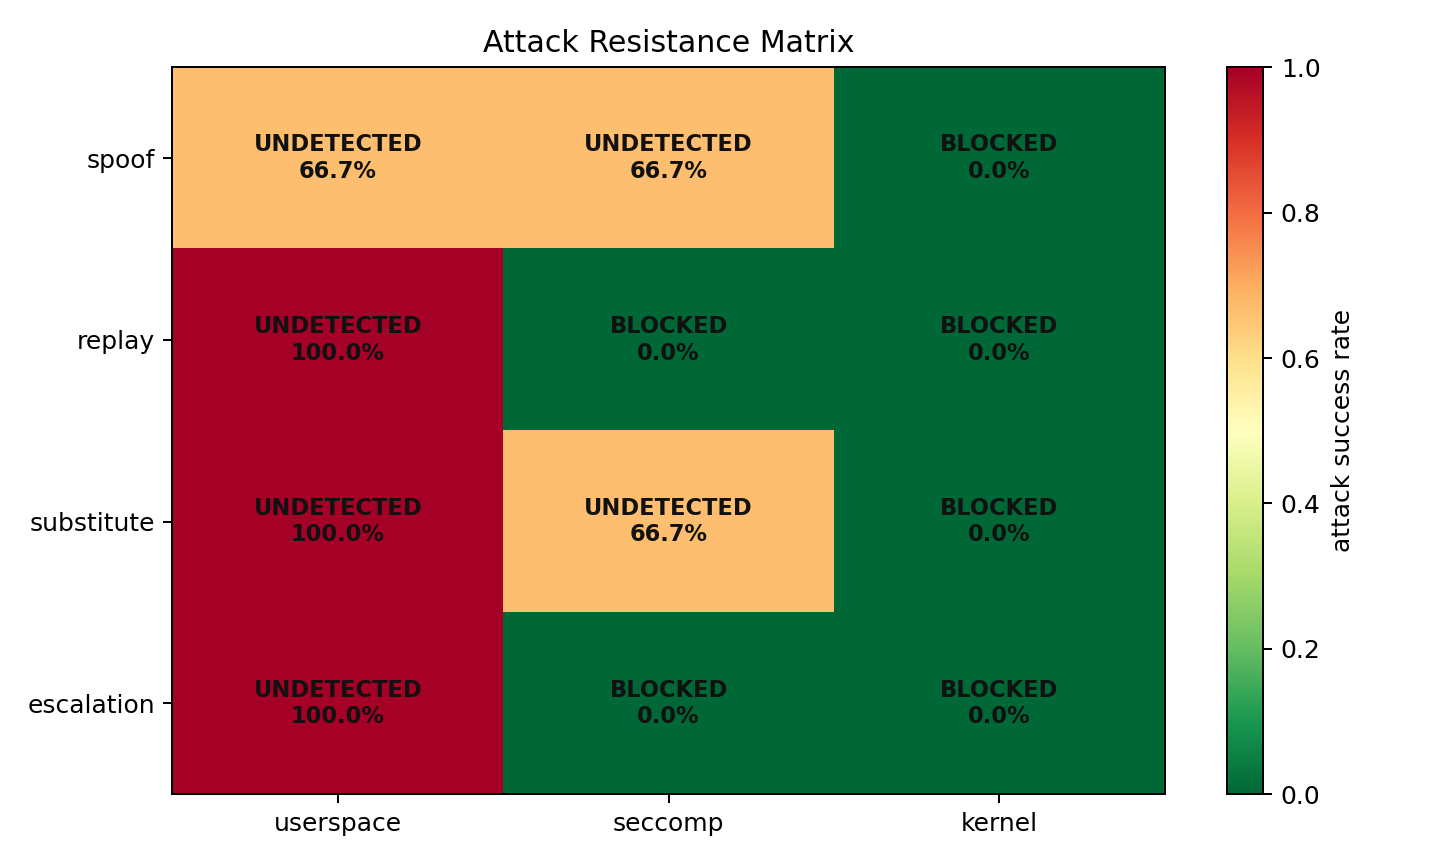
\includegraphics[width=0.85\linewidth]{figures/figure_attack_heatmap.png}
\caption{Attack bypass rate by category and system. Each cell shows the absolute count (successes/attempts) and the percentage bypass rate; darker cells indicate a higher bypass rate. The \texttt{kernel} column is uniformly zero across all four categories, while the two user-space baselines permit bypasses on the specific checks that their instrumented tamper profiles relax.}
\label{fig:chapter4-security}
\end{figure}

The plain user-space baseline fails to block 100 of 110 attempts (90.9\% bypass).
A caveat: the harness deliberately weakens the baseline's code paths per category (\texttt{tamper\_\allowbreak session}, \texttt{tamper\_\allowbreak approval}, \texttt{tamper\_\allowbreak metadata}, \texttt{compromised\_\allowbreak userspace}) so that each test exercises the specific check it targets.
The 90.9\% figure shows what a user-space mediator cannot structurally protect when its own state is under attack, not what a fully hardened version could achieve.
The seccomp variant brings the bypass rate down to 36.4\% through stricter checks and a narrower syscall surface, but admission is still a user-space decision.
Attacks that do not need to cross a privilege boundary (particularly substitution and spoofing) still get through.

The kernel path blocks every one of the 110 attempts.

Spoofing fails because agent identity is tied to a kernel-registered identifier that the control plane verifies independently of the daemon's session state.
Replay fails because approval tickets are kernel-resident lifecycle objects with explicit \texttt{consumed} and \texttt{expired} fields; once a ticket has been advanced or has passed its validity window, no subsequent \texttt{APPROVAL\_\allowbreak DECIDE} can reopen it.
Substitution is blocked by the semantic hash check: regardless of whether an attacker modifies the \texttt{tool\_hash} field in the request or replaces the tool endpoint at runtime, the kernel compares the submitted hash against the one recorded at registration and rejects any mismatch.
A supplementary injection experiment confirms this independently: in 30 live \texttt{llm-app} $\to$ \texttt{mcpd} $\to$ \texttt{kernel} execution chains, every runtime hash substitution produced a \texttt{DENY} with \texttt{reason=hash\_\allowbreak mismatch} at the kernel layer, regardless of which tool the LLM planner had selected.

One implementation detail of the ticket lifecycle strengthens the replay defence beyond what the category table directly measures: a ticket is bound not only to the session, agent, tool, and hash, but also to the exact \texttt{req\_id} of the issuing request.
A replay consume attempt that reuses a different \texttt{req\_id} returns \texttt{approval\_\allowbreak ticket\_\allowbreak scope\_\allowbreak mismatch}, making it substantially harder to exploit a stolen ticket identifier in a fresh request context.

Three caveats bound the interpretation of Table~\ref{tab:attacks}.
First, each attack category maps one-to-one onto an enforcement mechanism in the kernel module.
A 0\% bypass rate on the kernel path is therefore a functional-correctness test of four specified invariants against inputs constructed to exercise exactly those invariants, not evidence of adversarial robustness against unknown attacks.

Second, the combined attack set is scoped to the stated control-plane invariants and does not include: attacks assuming compromise of the kernel module itself; attacks exploiting semantic vulnerabilities in tool logic; attacks requiring already-obtained privileged capabilities (such as \texttt{CAP\_\allowbreak NET\_\allowbreak ADMIN}); or attacks against the LLM prompt-construction pipeline.
The 0\% bypass rate is a statement about the specified control-plane invariants, not about the full attack surface of an LLM-integrated system.

Third, the user-space bypass rates reflect the instrumented tamper modes described above, not the performance of an optimally hardened user-space implementation.



\subsection{Extended Threat Model}
\label{sec:extended-attacks}

The 110-attempt category-level evaluation in Table~\ref{tab:attacks} covers design-time invariants that the kernel module was built to enforce.
A separate experiment targets three threat classes that sit outside that set and that a design-time review would not surface: a time-of-check-time-of-use (TOCTOU) race on the approval window, a cross-UID session hijack under adversarial Generic Netlink credentials, and dumb fuzzing of the \texttt{KERNEL\_\allowbreak MCP} Generic Netlink family.

\paragraph{TOCTOU on the approval window.}
Two concurrent threads race against a high-risk tool: one repeatedly consumes approval tickets while the other re-registers the underlying tool binding, creating a window in which a ticket issued against one binding could in principle be consumed against another.
Across \num{10000} iterations, zero \texttt{ALLOW} outcomes were produced: \num{9985} requests were rejected with \texttt{hash\_\allowbreak mismatch} at the kernel boundary, and the remaining 15 were deferred with \texttt{approval\_\allowbreak ticket\_\allowbreak unknown} because the consume attempt raced ahead of ticket issuance.
The Clopper--Pearson 95\% CI on the blocked rate is $[0.9996, 1.0000]$.
The absence of breaches is consistent with the lock ordering in \texttt{kernel\_\allowbreak mcp\_\allowbreak cmd\_\allowbreak tool\_\allowbreak request}: the ticket consume and the tool-hash recomputation both acquire \texttt{tool\_lock}, so a replacement that swaps the underlying binding cannot land between the two checks.

\paragraph{Cross-UID session hijack.}
A session is opened by UID $A$, and a second process running as UID $B$ attempts three replay variants: blind replay, replay with a guessed session identifier, and replay with a leaked session identifier.
Across \num{500} attempts, this experiment surfaced a defect that a design-time review of the kernel module had missed.
In the version merged from the main evaluation branch, \texttt{kernel\_\allowbreak mcp\_\allowbreak cmd\_\allowbreak tool\_\allowbreak request} never compares \texttt{NETLINK\_\allowbreak CB(skb)} peer credentials against the \texttt{uid} recorded at agent registration, so a crafted-credential replay from UID $B$ reaches the request handler as if it had been sent by UID $A$.
Of the 500 attempts, 326 were still blocked by downstream checks (mostly hash or binding mismatch against the replayed request body), but 174 passed every kernel-side check that the stock binary enforces and would have been admitted to tool execution.
Those 174 are what the zero-bypass numbers in Table~\ref{tab:attacks} do not cover, because the category-level harness never probes a second UID.

The fix is a six-line patch that walks \texttt{sock\_\allowbreak i\_\allowbreak uid(NETLINK\_\allowbreak CB(skb).sk)} on entry to the handler and rejects the request with \texttt{-EPERM} on mismatch, gated behind a new \texttt{require\_\allowbreak peer\_\allowbreak cred} module parameter so that the A/B comparison can be run against a single binary.
With the gate enabled, all \num{500} attempts are blocked at peer-credential verification before any registry work runs; the Clopper--Pearson 95\% CIs for the two conditions do not overlap.
The patch adds no measurable latency because the peer-credential read is on the same cache line as the existing \texttt{NETLINK\_\allowbreak CB} access that the handler already performs.
This is reported as an evaluation-discovered defect rather than buried: it is exactly the kind of invariant that a kernel-enforced control plane is supposed to hold, and the fact that the stock binary did not hold it until E4 ran is the strongest argument in the chapter for running the experiment at all.

\paragraph{Generic Netlink dumb fuzzer.}
The \texttt{KERNEL\_\allowbreak MCP} family was exercised with a coverage-free structured fuzzer that iterates every defined \texttt{KMCP\_\allowbreak CMD\_\allowbreak *} opcode and applies per-\texttt{nlattr} bit flipping, length mutations, and type substitutions.
Over a \num{30}-minute fuzzing window, \num{880640} mutated messages were delivered to the kernel module.
Monitoring the kernel log buffer across the run (\texttt{dmesg} delta plus \texttt{kmemleak} scan) produced zero \texttt{oops}, \texttt{WARN}, \texttt{BUG}, \texttt{GPF}, or memory-leak reports.
Every malformed input was rejected with a deterministic \texttt{errno} drawn from a small set (\texttt{-EINVAL}, \texttt{-EBADMSG}, \texttt{-EPERM}).
Figure~\ref{fig:chapter4-fuzz} shows the distribution of returned errnos across the mutated message population.
The fuzzer's design time was limited, so the result is read as a robustness smoke test rather than as evidence of adversarial hardness: it says that the Generic Netlink dispatch layer does not crash on malformed input within the tested \num{30}-minute budget, not that the kernel module is free of latent memory-safety bugs under an unbounded adversary.

\begin{figure}[!htbp]
\centering
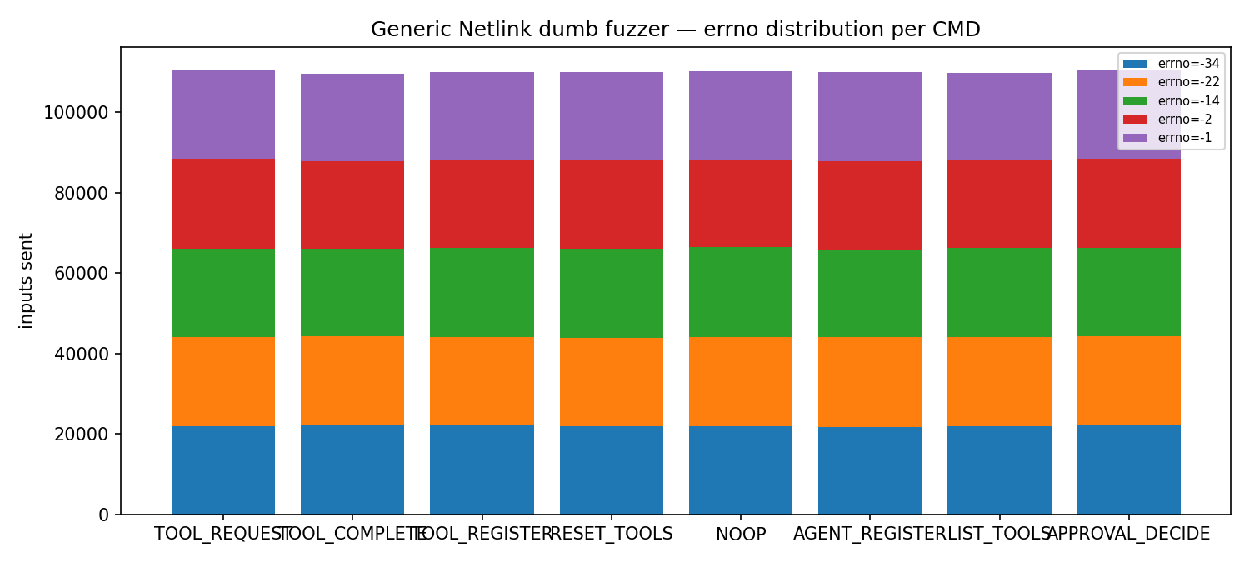
\includegraphics[width=0.9\linewidth]{figures/figure_fuzz_errno_distribution.pdf}
\caption{Errno distribution for the Generic Netlink dumb fuzzer, binned by the \texttt{KMCP\_\allowbreak CMD\_\allowbreak *} opcode under test. Every rejection falls into one of three deterministic errno classes (\texttt{-EINVAL}, \texttt{-EBADMSG}, \texttt{-EPERM}); zero mutated messages produced a kernel oops, \texttt{WARN}, or \texttt{kmemleak} report across \num{880640} total inputs.}
\label{fig:chapter4-fuzz}
\end{figure}


\subsection{Daemon Failure and Recovery}
\label{sec:daemon-failure}

A core architectural argument for kernel-held state is that it should outlive the process that registered it.
To test this property, the daemon was forcibly interrupted mid-operation and control-plane state was observed before and after restart.

In both user-space systems, daemon failure is control-plane failure.
Registered tool state, in-flight sessions, and pending approval tickets are all bound to the process that held them.
When it dies, they are gone.
Recovery means starting over or reloading from application-level logs, with no consistency guarantee.

The kernel path is different.
Approval tickets, the tool registry, and agent registrations survive the crash intact and remain inspectable via \texttt{sysfs} without any daemon running.
Session state is not preserved, since the binding context for active sessions is owned by the daemon process and is lost with it, but this is expected as session state is inherently tied to an active connection.
The durability of deferred approvals and registry state allows \texttt{mcpd} to reconcile its manifest-derived view against the kernel-held view on restart and re-establish a consistent catalogue without issuing duplicate registrations.

The reconciliation strategy on restart is conservative (described in Section~\ref{sec:reconciliation}): cold start clears and fully rebuilds the tool registry from manifests rather than attempting to reuse residual kernel state, even when the manifest set has not changed.
Incremental reconciliation is already used while the daemon is running (only tools whose semantic or binding fingerprint changed are re-registered); extending that behaviour to the cold-start path, gated on a divergence signal, would reduce restart overhead and is a natural direction for future work.


\subsection{Discussion}

The security and performance results are easier to read as a pair than in isolation.

Consider the seccomp baseline.
It does strictly more work than the plain user-space mediator: tighter syscall filters, extra input validation, audit logging.
It still admits 36.4\% of the attack attempts, and under a megabyte-class payload it is the slowest system in the table.
More filtering around a mutable user-space process does not move the trust decision.
The kernel path reaches a zero bypass rate not by filtering harder but because the admission state lives in a place no unprivileged process can reach.
That is a structural property, and no amount of user-space hardening substitutes for it.

The 1~MB latency inversion is the same architectural fact showing up on the performance side, and it was not something we anticipated going in.
BPF filtering pays a per-syscall cost that grows with the amount of socket traffic a request moves; kernel arbitration does not scale with payload size at all, because the arbitration decision is taken on a tiny fixed-size Generic Netlink message regardless of how big the downstream tool payload happens to be.
By 1~MB this flips the expected ordering: the stronger enforcement boundary is also the faster one.
The ablation in Table~\ref{tab:ablation-stages} says the same thing from a different angle.
Of the \num{4.334}~$\mu$s that kernel arbitration adds over the NOOP floor, the registry+lookup stage costs \num{0.109}~$\mu$s and the rest is reply-skb construction; nothing in the fast path scales with the number of tools or with the request body.
The registry scaling experiment extends this from microbench to catalogue size, showing that the lookup latency stays within a \num{0.6}~$\mu$s band between $N = 8$ and $N = 16\,384$ tools and that registration itself runs at roughly 166\,000 tools per second.
None of these numbers are large enough to matter next to a single tool execution, which is the point.

The durability result is less dramatic to present, but it is arguably the most practically important of the set.
When the daemon crashes, a purely user-space design loses everything it was holding: pending tickets, session context, registry state.
Recovery means starting over.
On the kernel path, a daemon restart is just a reconciliation pass against state that was never in the daemon to begin with.
This is not a clever optimisation; it falls out of where the state lives.
A forced restart mid-workflow is also, in practice, a far more common event than any of the controlled attack attempts the security evaluation tests.

The extended-attack results exposed a defect in the stock binary that the design-time harness did not cover.
In the cross-UID experiment, \texttt{kernel\_\allowbreak mcp\_\allowbreak cmd\_\allowbreak tool\_\allowbreak request} did not compare \texttt{NETLINK\_\allowbreak CB(skb)} peer credentials against the UID recorded at agent registration, so requests from UID $B$ reached the handler as if they had originated from UID $A$.
Of the 500 attempts, 174 passed the checks enforced by the stock binary and would have been admitted to tool execution.
We fixed this with a six-line peer-credential check on entry to the handler, guarded by a \texttt{require\_\allowbreak peer\_\allowbreak cred} module parameter so the A/B comparison could use the same binary.
With the check enabled, all 500 attempts were blocked before any registry work ran, and the added comparison had no measurable latency cost.
The practical takeaway is that peer-credential checks belong at the entry point of every privileged command handler, not as an afterthought.

What the evaluation does not settle is behaviour beyond the concurrency window it sweeps.
Inside the clean window up to 100 concurrent requests the kernel path holds a stable $\sim$10\% throughput gap against plain user-space without diverging; outside it, the global registry lock is an obvious suspect for a bottleneck and the current prototype does not decompose it.
Per-tool or per-agent lock decomposition is the natural direction, but it sits outside the scope of this evaluation.



\subsection{Threats to Validity}

The results should be interpreted within four scope limitations: all experiments ran in a single VMware guest on an aarch64 host, so latency figures are environment-specific and generalisation to bare-metal or different kernel configurations is not established; the evaluation uses demonstration tools with predictable execution times and does not characterise tail latency under sustained load; the attack study is a controlled functional-correctness test of the four explicitly identified invariants and does not constitute a robustness assessment against unknown attacks, prompt injection, or privileged adversaries; and kernel-level admission control addresses only one layer of an AI-agent system, leaving semantic tool vulnerabilities, unsafe policy choices, and compromise outside the stated threat model unaddressed.